\chapter{Analysis}
\label{analysis}
 %spacje przed cytowaniami, sprawdź "palsy"
Before describing the possible solution for the problem of rehabilitation for children with dyspraxia, an introduction about the disorder itself as well as its treatment methods and difficulties connected with them will be made. %TODO "should be made" - should be replaced with a better word

\section{Developmental coordination disorder (dyspraxia)}

Developmental Coordination Disorder (DCD), also known as \emph{developmental dyspraxia}, is the inability to plan, organise and coordinate movement \cite{4}. It results in fine and gross motor problems and/or speech difficulties, which can have strong negative impact on daily activities and academic achievements. Dyspraxia was first described by WHO in 1992. It is a hard to diagnose and even harder to cure motor disorder, which is subcategory of neurodevelopmental disorder – along with autism and Down syndrome - and mostly identified among children. It often appears together with neurological illnesses from other subcategories, like ADHD, Asperger syndrome or dyslexia \cite{20}. It is, however, also sporadically detected in completely healthy (except for DCD) children who are developing well intellectually \cite{20}. DCD is not caused by motor or sensory impairments, similar to muscular dystrophy or Parkinson's disease. No correlation to any known neurological condition or intellectual impairment could be found.

\section{Prevalence}
DCD’s prevalence range from 5\% to 15\% in the primary school and it is confirmed that about 5\% of all children are affected, but not all of them have a severe case of DCD \cite{20}. Children born prematurely \cite{1} and children with extremely low birth weights \cite{21} are at a significantly increased risk of having DCD. According to the majority of researches prevalence ratio is about 4:1 in boys than girls, but it is not confirmed - it differs between 5:1 to even 2:1 depending on study \cite{20}. There are hypotheses that so high and unproven proportion is connected with the fact, that the frequent presence of comorbid conditions (e.g. ADHD) can make DCD easier to identify among boys. %TODO next sentence needs work
Also, girls do not have so strict social requirements regarding motor skills – therefore being clumsy may not be perceived as a disorder. 
Moreover, the majority of the children do not "grow out of" this disorder and it persists into adulthood.

\section{Symptoms}
There are numerous signs and symptoms of developmental dyspraxia as each case can be very distinct. The most noticeable ones are those connected with coordination and movement. Typically, representative symptoms of DCD are:

\begin{itemize} [noitemsep]
\item difficulty in combining movements into controlled sequence,
\item remembering the next movement in sequence,
\item poor timing and disturbed balance.
\end{itemize}

The common cause for all of the above and other movement problems is working memory dysfunction.
Working memory, often used synonymously with short-term memory, is the system in the brain which manipulates all "current data" - visual images or verbal information - and coordinates the central executive. 
One of the crucial responsibilities of the latter is creating a visual representation of possible movement paths. 
If this subsystem does not work properly, the patient will not perform his movements accurately. 

Problems with working memory may have deep impact on patient's abilities and skills. It may result in having difficulties remembering deadlines and sequences of instructions, like cooking, driving a car or playing complex games. However, this disorder does not affect one's long-term memory, which actually can be excellent, despite poor short-time memory.

There are many more possible symptoms of DCD:

\begin{itemize} [noitemsep]
\item problems with spatial awareness, 
\item determining left or right, 
\item estimating the distance to objects.
\end{itemize} 

Fine motor problems can occur, i.e. difficulty in acquisition of graphemes (e.g. letters or numbers – that is why people with dyspraxia also sometimes suffer from dysgraphia or dyslexia) or establishing an efficient pencil grip.

\section{Real-life impact}
To conclude the description of disease, it is crucial to determine its impact on real-life activities. Issues with motor coordination may cause problems with walking, running, climbing or jumping. Working memory problems can lead to having difficulties driving a car, moving in crowded places, crossing roads and make a person prone to panic attacks. People with DCD are facing difficulties using cutlery, fastening buttons or shoelaces, shaving and performing similar routine activities. In conclusion, if the disorder is not cured, it may be extremely demanding on the patient.

\section{Diagnosing}
Although the disease is strictly neurological, researches about detecting DCD with imaging techniques like computed tomography, magnetic resonance imaging or ultrasound are inconclusive \cite{3}. %TODO next sentence needs rewriting, or proper quotation
Several theories speculate that the etiology of DCD is part of the continuum of cerebral palsy; is secondary to prenatal, perinatal, or neonatal insult; or is secondary to neuronal damage at the cellular level in the neurotransmitter or receptor systems \cite{5}. Experiments and researches in this topic are ambiguous and cannot be a basis for definitive diagnosis.

The most popular and conclusive way of diagnosing DCD is to perform a standardized motor test. A score below 15th percentile and IQ above 69 points qualifies the patient for a diagnosis of DCD \cite{22}. However, there is some inconsistency among tests. In one study \cite{10}, two tests were compared - the Bruininks-Oseretsky Test of Motor Proficiency (BOTMP) and the Movement Assesment Battery for Children(M-ABC). The tested group consists of children with DCD and with no motor difficulties in 1:1 proportion. The size of test group was 312 in the first trial and 202 in the second. The test results shown respectively 82\% and 67\% consistency in distinguishing children who had DCD from children who did not \cite{5}. Those are two of the most commonly used tests for diagnosing DCD - the potential lack of consistency in identifying DCD among children is a serious concern.

In the majority of cases, the diagnosis is based on observation of signs and symptoms. The American Psychiatric Association considers that DCD should be diagnosed only if the following four diagnostic components are present \cite{14}:
\begin{itemize} [noitemsep]
\item Motor coordination during daily activities should be substantially below that expected for age and intelligence.
\item Resulting motor difficulties interfere with academic achievement or activities of daily living.
\item The coordination problems are not due to a general medical condition (e.g., cerebral palsy or muscular dystrophy) or a pervasive developmental disorder.
\item If mental retardation is present, the motor difficulties are in excess of those usually associated with mental retardation.
\end{itemize}

\section{Treatment}
The treatment for DCD is based on rehabilitation and training. No pharmacological therapy was designed to be used during DCD's treatment. Medications are reserved for the treatment of associated conditions (e.g., attention deficit hyperactivity disorder[ADHD]) \cite{12}. 

There are two basic approaches of rehabilitation procedure - top-down and bottom-up. Top-down approach, also known as task-oriented or modular, attempts to remedy or improve specific difficulties by employing specific techniques aimed at the observed motor challenge (e.q., difficulty with handwriting, catching a ball, or performing fine motor tasks with the fingers). It usually involves gradually targeting certain problem behaviours and implementing step-by-step interventions that focus on teaching and practising the skill \cite{12}. The most important element of modular-approach is practice. Practical applications of this method are therapies such as the cognitive motor approach with task orientation or task-oriented approaches with motor learning.

Bottom-up approach (process-oriented, deficit-oriented), the more global or generalised one is based on the theoretical assumption that the motor skills problem is just a manifestation of some underlying mechanism, such as impaired sensory integration or insufficient or inaccurate kinaesthetic perceptions. In the bottom-up approach, the therapist does not initially address the observable motor challenge. Rather, the expert focuses on how children manage their bodies, process stimulation (sensory information), and deal with problems. The expectation is that the improved sensory-motor (sensorimotor) functioning becomes generalized and eventually improves the motor skills. As children become comfortable with their bodies, they gain control of their motor (and other) functions \cite{12}. This method is represented by the kinaesthetic training approach, sensorimotor integration therapy and sensory integration therapy. 

No researches show that any of this approaches is definitely effective as DCD's treatment. This is probably caused by great diversity in symptoms and severity's levels of DCD. However, data suggest that top-down approach may be more efficient than bottom-up.


\section{Haptic devices in rehabilitation}
There are researches that prove the sensorimotor control of limb stiffness and compliance is a key element in the organisation of movement. Though, the best training approach would be the sensorimotor training. The goal of this therapy is to improve child's perceptual abilities intrinsic to the concurrent generation and experience of their own movements as well as use of this information to guide their movements \cite{13}.

This kind of training is difficult to apply with traditional therapeutic tools. However, various robot-assisted therapies are developed in order to support sensorimotor training, some of them including haptic devices. Robot-assisted therapies allowed to perform rehabilitation without the direct supervision of a trained therapist, what is especially important in DCD, where the number of patients significantly outgrows number of therapists. What's more, the complexity or/and difficulty of the task can be controlled very precisely. 

Haptic devices were used to improve the generation of handwriting movements of children with DCD \cite{9}. The researches show that this method can be notably effective, mostly because of active sensorimotor generation and control of movement trajectories. This is the feature required for learning generalized to task-related movements other than those specifically practised \cite{13}. This requirement is caused by "catch-22" situation connected with movement learning mechanism. This learning process for a person without dyspraxia consists of two stages. First one is learning to generate imprecise approximation of movement. When this is achieved, one can gradually improve approximation of a movement through practice until achieving optimal route. For people with dyspraxia it is almost impossible to generate generate good enough qualitative approximation, which should allow them to make quantitative improvements through practice - this is a "catch-22". 

It is possible to overcome this paradox only if the support from the machine is balanced with possibility of active generation and control of movement from child. Mechanical properties of haptic devices, like inertia and tactile feedback can significantly help in achieving this result \cite{13}.
 
\section{Haptic factors essential for rehabilitation. Phantom Omni description.}
\label{phantom_introduction} 

\begin{wrapfigure}{L} {0.5\textwidth}
\begin{center}
	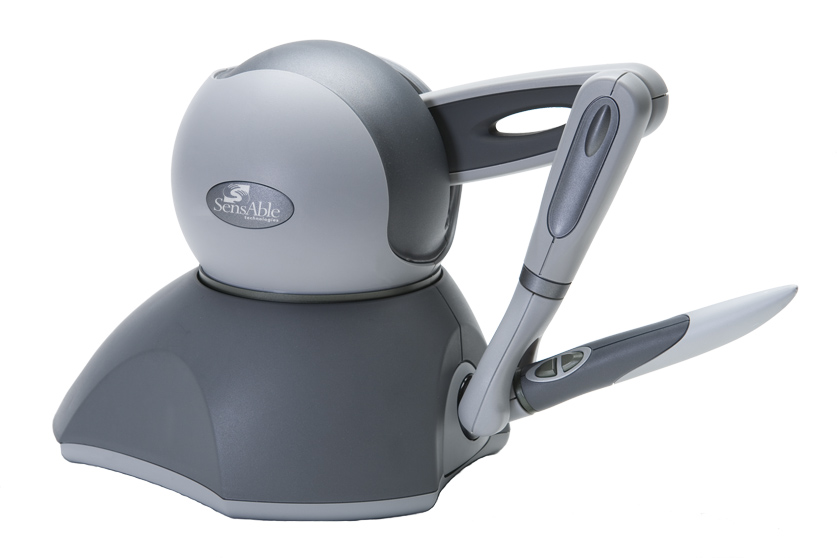
\includegraphics[width=5cm]{Images/phantom_basic}
	\label{fig:phantom_basic}	
	\caption{Sensable Phantom Omni device}
\end{center}
\end{wrapfigure}
Using haptic devices as controllers in application allows to benefit from the various haptic factors generated by particular haptic device. The factors vary between products and producers. Because all of quotable studies operate on Sensable Phantom Omni(Geomagic Touch Haptic Device) \cite{8}, when "haptic device" will be mentioned in text, it will always refer to Phantom device. 

Phantom Omni (\ref{fig:phantom_basic} - \nameref{fig:phantom_basic}) consists of stylus connected to an arm mounted on base. It has 6 degrees of freedom and its workspace range is 160x120x70mm. Thanks to its pen-like stylus it is easy and natural to operate it, especially for children. Phantom Omni has been widely used in industry for a several years, also for medical purposes, thus it is well tested and safe-in-use device.

The haptic factors generated by this device and tested in children's rehabilitation are \cite{9} \cite {13}:
\begin{itemize} [noitemsep]
\item inertia,
\item viscosity (of the space),
\item magnetic attraction of the object),
\item friction  (of the object).
\end{itemize}
Viscosity and inertia may provide an appropriate support, but do not allow to keep track of designed movement form. Furthermore, no evidence suggest that the method could generalize the performance without support from the device \cite{9}. Magnetic attraction help in following the generated path and this is the main haptic factor that will be used in the project. Researches show that friction has no significant impact on helping the child in performing the task \cite{13}.

\section{Game rules analysis}
\label{rules}
In order to develop a serious game which can help children with dyspraxia, some basic rules and presumption must be established. The following principles are based either on \cite{13}, where similar project was developed or on the top of previous subsections analysis:
\begin{enumerate} [noitemsep]
\item The game represents a bottom-up approach with sensorimotor training.
\item Basic task is to follow the path with tip of stylus, where the path is magnetically attractive.
\item The main haptic factor is magnetic attraction.
\item There must exists a levelling system.
\end{enumerate}

The next chapter describes the design phase of a game based on this rules. 